%\documentclass[a4paper]{article}
\documentclass[10pt,landscape,a4paper]{article}
% Этот шаблон документа разработан в 2014 году
% Данилом Фёдоровых (danil@fedorovykh.ru) 
% для использования в курсе 
% <<Документы и презентации в \LaTeX>>, записанном НИУ ВШЭ
% для Coursera.org: http://coursera.org/course/latex .
% Исходная версия шаблона --- 
% https://www.writelatex.com/coursera/latex/5.3

% В этом документе преамбула

\usepackage{siunitx}
%%% Работа с русским языком
%\usepackage{cmap}					% поиск в PDF
%\usepackage{mathtext} 				% русские буквы в формулах
%\usepackage[T2A]{fontenc}			% кодировка
%\usepackage[utf8]{inputenc}			% кодировка исходного текста
%\usepackage[english,russian]{babel}	% локализация и переносы
%\usepackage{indentfirst}
%\frenchspacing
%
%\renewcommand{\epsilon}{\ensuremath{\varepsilon}}
%\newcommand{\phibackup}{\ensuremath{\phi}}
%\renewcommand{\phi}{\ensuremath{\varphi}}
%\renewcommand{\varphi}{\ensuremath{\phibackup}}
%\renewcommand{\kappa}{\ensuremath{\varkappa}}
%\renewcommand{\le}{\ensuremath{\leqslant}}
%\renewcommand{\leq}{\ensuremath{\leqslant}}
%\renewcommand{\ge}{\ensuremath{\geqslant}}
%\renewcommand{\geq}{\ensuremath{\geqslant}}
%\renewcommand{\emptyset}{\varnothing}
%\renewcommand{\Im}{\operatorname{Im}}
%\renewcommand{\Re}{\operatorname{Re}}


%%% Дополнительная работа с математикой
\usepackage{amsmath,amsfonts,amssymb,amsthm,mathtools} % AMS
%\usepackage{icomma} % "Умная" запятая: $0,2$ --- число, $0, 2$ --- перечисление

%% Номера формул
%\mathtoolsset{showonlyrefs=true} % Показывать номера только у тех формул, на которые есть \eqref{} в тексте.
%\usepackage{leqno} % Нумереация формул слева

%% Свои команды
\DeclareMathOperator{\sgn}{\mathop{sgn}}
\DeclareMathOperator{\sign}{\mathop{sign}}
\DeclareMathOperator*{\res}{\mathop{res}}
\DeclareMathOperator*{\tr}{\mathop{tr}}
\DeclareMathOperator*{\rot}{\mathop{rot}}
\DeclareMathOperator*{\divop}{\mathop{div}}
\DeclareMathOperator*{\grad}{\mathop{grad}}

%% Перенос знаков в формулах (по Львовскому)
\newcommand*{\hm}[1]{#1\nobreak\discretionary{}
{\hbox{$\mathsurround=0pt #1$}}{}}

%%% Работа с картинками
\usepackage{graphicx}  % Для вставки рисунков
\graphicspath{{figures/}}  % папки с картинками
\setlength\fboxsep{3pt} % Отступ рамки \fbox{} от рисунка
\setlength\fboxrule{1pt} % Толщина линий рамки \fbox{}
\usepackage{wrapfig} % Обтекание рисунков текстом

%%% Работа с таблицами
\usepackage{array,tabularx,tabulary,booktabs} % Дополнительная работа с таблицами
\usepackage{longtable}  % Длинные таблицы
\usepackage{multirow} % Слияние строк в таблице

%%% Теоремы
\theoremstyle{plain} % Это стиль по умолчанию, его можно не переопределять.
\newtheorem{thm}{Теорема}
\newtheorem*{thm*}{Теорема}
\newtheorem{prop}{Предложение}
\newtheorem*{prop*}{Предложение}
 
\theoremstyle{definition} % "Определение"
%\newtheorem{corollary}{Следствие}[theorem]
\newtheorem{dfn}{Определение}
\newtheorem*{dfn*}{Определение}
\newtheorem{prob}{Задача}
\newtheorem*{prob*}{Задача}

 
\theoremstyle{remark} % "Примечание"
\newtheorem*{sol}{Решение}
\newtheorem*{rem}{Замечание}

%%% Программирование
\usepackage{etoolbox} % логические операторы

%%% Страница
%\usepackage{extsizes} % Возможность сделать 14-й шрифт
%\usepackage{geometry} % Простой способ задавать поля
%	\geometry{top=25mm}
%	\geometry{bottom=35mm}
%	\geometry{left=35mm}
%	\geometry{right=20mm}
 
\usepackage{fancyhdr} % Колонтитулы
%	\pagestyle{fancy}
 %	\renewcommand{\headrulewidth}{0pt}  % Толщина линейки, отчеркивающей верхний колонтитул
	%\lfoot{Нижний левый}
	%\rfoot{Нижний правый}
	%\rhead{Верхний правый}
	%\chead{Верхний в центре}
	%\lhead{Верхний левый}
	%\cfoot{Нижний в центре} % По умолчанию здесь номер страницы

\usepackage{setspace} % Интерлиньяж
%\onehalfspacing % Интерлиньяж 1.5
%\doublespacing % Интерлиньяж 2
%\singlespacing % Интерлиньяж 1

\usepackage{lastpage} % Узнать, сколько всего страниц в документе.

\usepackage{soul} % Модификаторы начертания

\usepackage{hyperref}
\usepackage[usenames,dvipsnames,svgnames,table,rgb]{xcolor}
\hypersetup{				% Гиперссылки
    unicode=true,           % русские буквы в раздела PDF
    pdftitle={Заголовок},   % Заголовок
    pdfauthor={Автор},      % Автор
    pdfsubject={Тема},      % Тема
    pdfcreator={Создатель}, % Создатель
    pdfproducer={Производитель}, % Производитель
    pdfkeywords={keyword1} {key2} {key3}, % Ключевые слова
%    colorlinks=true,       	% false: ссылки в рамках; true: цветные ссылки
    %linkcolor=red,          % внутренние ссылки
    %citecolor=black,        % на библиографию
    %filecolor=magenta,      % на файлы
    %urlcolor=cyan           % на URL
}

\usepackage{csquotes} % Еще инструменты для ссылок

%\usepackage[style=apa,maxcitenames=2,backend=biber,sorting=nty]{biblatex}

\usepackage{multicol} % Несколько колонок

\usepackage{tikz} % Работа с графикой
\usepackage{pgfplots}
\usepackage{pgfplotstable}
%\usepackage{coloremoji}
\usepackage{floatrow}
\usepackage{subcaption}
\graphicspath{{figures/}}

\renewcommand\thesubfigure{\asbuk{subfigure}}
%\addbibresource{master.bib}

\usepackage{import}
\usepackage{pdfpages}
\usepackage{transparent}
\usepackage{xcolor}
\usepackage{xifthen}

\newcommand{\incfig}[2][1]{%
    \def\svgwidth{#1\columnwidth}
    \import{./figures/}{#2.pdf_tex}
}
%\usepackage{titlesec}
%\titleformat{\section}{\normalfont\Large\bfseries}{}{0pt}{}
%----------------------STANDART:
%\titleformat{\chapter}[display]
%  {\normalfont\huge\bfseries}{\chaptertitlename\ \thechapter}{20pt}{\Huge}
%\titleformat{\section}{\normalfont\Large\bfseries}{\thesection}{1em}{}
%\titleformat{\subsection}
%  {\normalfont\large\bfseries}{\thesubsection}{1em}{}
%\titleformat{\subsubsection}
%  {\normalfont\normalsize\bfseries}{\thesubsubsection}{1em}{}
%\titleformat{\paragraph}[runin]
%  {\normalfont\normalsize\bfseries}{\theparagraph}{1em}{}
%\titleformat{\subparagraph}[runin]
%  {\normalfont\normalsize\bfseries}{\thesubparagraph}{1em}{}

\pdfsuppresswarningpagegroup=1
\pgfplotsset{compat=1.16}



%\setcounter{tocdepth}{1} % only parts,chapters,sections
%\titleformat{\subsection}{\normalfont\large\bfseries}{}{0em}{}
%\titleformat{\subsubsection}{\normalfont\normalsize\bfseries}{}{0em}{}

%\newcommand{\textover}[2]{\stackrel{\mathclap{\normalfont\mbox{#2}}}{#1}}

\author{Yaroslav Drachov\\
Moscow Institute of Physics and Technology}
%\author{Драчов Ярослав\\
%Факультет общей и прикладной физики МФТИ}
\newcommand{\veq}{\mathrel{\rotatebox{90}{$=$}}}
%\newcommand{\teto}[1]{\stackrel{\mathclap{\normalfont\tiny\mbox{#1}}}{\to}}
%\renewcommand{\thesubsection}{\arabic{subsection}}

%%\setcounter{secnumdepth}{0}

\definecolor{tabblue}{RGB}{30, 119, 180}
\definecolor{taborange}{RGB}{255, 127, 15}
\definecolor{tabgreen}{RGB}{45, 160, 43}
\definecolor{tabred}{RGB}{214, 38, 40}
\definecolor{tabpurple}{RGB}{148, 103, 189}
\definecolor{tabbrown}{RGB}{140, 86, 76}
\definecolor{tabpink}{RGB}{227, 119, 193}
\definecolor{tabgray}{RGB}{127, 127, 127}
\definecolor{tabolive}{RGB}{188, 189, 33}
\definecolor{tabcyan}{RGB}{22, 190, 207}
\pgfplotscreateplotcyclelist{colorbrewer-tab}{
{tabblue},
{taborange},
{tabgreen},
{tabred},
{tabpurple},
{tabbrown},
{tabpink},
{tabgray},
{tabolive},
{tabcyan},
}
\usepackage{csvsimple}
\usepackage{extarrows}
%\renewcommand{\labelenumii}{\asbuk{enumii})}
%\renewcommand{\labelenumiv}{\Asbuk{enumiv}}
%\newcommand{\prob}[1]{\subsubsection*{#1}}
\sisetup{output-decimal-marker = {,},separate-uncertainty = true,exponent-product = \cdot}

\usepackage{braket}
\usepackage{enumerate}
\usepackage{chngcntr}
%\counterwithin*{equation}{problem}
%\usepackage{bbold}

\newtheoremstyle{hiProb}% ⟨name ⟩ 
{3pt}% ⟨Space above ⟩1 
{3pt}% ⟨Space below ⟩1
{}% ⟨Body font ⟩
{}% ⟨Indent amount ⟩2
{\bfseries}% ⟨Theorem head font⟩
{.}% ⟨Punctuation after theorem head ⟩
{.5em}% ⟨Space after theorem head ⟩3
%{\thmname{#1} \thmnote{#3}}% ⟨Theorem head spec (can be left empty, meaning ‘normal’)⟩
{\thmnote{#3}}% ⟨Theorem head spec (can be left empty, meaning ‘normal’)⟩
\theoremstyle{hiProb} % "Определение"
%\newtheorem{hiProb}{Задача}
\newtheorem{hiProb}{}
%\usepackage{mmacells}
\newcommand{\textover}[2]{\stackrel{\mathclap{\normalfont\scriptsize\mbox{#2}}}{#1}}
\usepackage{units}
\usepackage[math]{cellspace}%
\setlength\cellspacetoplimit{2pt}
\setlength\cellspacebottomlimit{2pt}

\DeclareMathAlphabet{\mathbbold}{U}{bbold}{m}{n}

\newcommand{\normord}[1]{:\mathrel{#1}:}

%\titleformat{\section}
%  {\normalfont\normalsize\bfseries}{\thesection}{1em}{}
%\titlespacing\section{0pt}{12pt plus 4pt minus 2pt}{0pt plus 2pt minus 2pt}
%\pagenumbering{gobble}
%\title{Дебильник}
\usepackage{tikz}
\usetikzlibrary{shapes,positioning,arrows,fit,calc,graphs,graphs.standard}
%\usepackage[nosf]{kpfonts}
%\usepackage[t1]{sourcesanspro}
%\usepackage[lf]{MyriadPro}
%\usepackage[lf,minionint]{MinionPro}
\usepackage{multicol}
\usepackage{wrapfig}
\usepackage[top=0mm,bottom=1mm,left=0mm,right=1mm]{geometry}
\usepackage[framemethod=tikz]{mdframed}
\usepackage{microtype}

\let\bar\overline

\definecolor{myblue}{cmyk}{1,.72,0,.38}

\def\firstcircle{(0,0) circle (1.5cm)}
\def\secondcircle{(0:2cm) circle (1.5cm)}

\colorlet{circle edge}{myblue}
\colorlet{circle area}{myblue!5}

\tikzset{filled/.style={fill=circle area, draw=circle edge, thick},
    outline/.style={draw=circle edge, thick}}

\pgfdeclarelayer{background}
\pgfsetlayers{background,main}

\everymath\expandafter{\the\everymath \color{myblue}}
\everydisplay\expandafter{\the\everydisplay \color{myblue}}

\renewcommand{\baselinestretch}{.8}
\pagestyle{empty}

\global\mdfdefinestyle{header}{%
linecolor=gray,linewidth=1pt,%
leftmargin=0mm,rightmargin=0mm,skipbelow=0mm,skipabove=0mm,
}

\newcommand{\header}{
\begin{mdframed}[style=header]
\footnotesize
\sffamily
Дебильник
\end{mdframed}
}

\makeatletter
\renewcommand{\section}{\@startsection{section}{1}{0mm}%
                                {.2ex}%
                                {.2ex}%x
                                {\color{myblue}\sffamily\small\bfseries}}
\renewcommand{\subsection}{\@startsection{subsection}{1}{0mm}%
                                {.2ex}%
                                {.2ex}%x
                                {\sffamily\bfseries}}



\def\multi@column@out{%
   \ifnum\outputpenalty <-\@M
   \speci@ls \else
   \ifvoid\colbreak@box\else
     \mult@info\@ne{Re-adding forced
               break(s) for splitting}%
     \setbox\@cclv\vbox{%
        \unvbox\colbreak@box
        \penalty-\@Mv\unvbox\@cclv}%
   \fi
   \splittopskip\topskip
   \splitmaxdepth\maxdepth
   \dimen@\@colroom
   \divide\skip\footins\col@number
   \ifvoid\footins \else
      \leave@mult@footins
   \fi
   \let\ifshr@kingsaved\ifshr@king
   \ifvbox \@kludgeins
     \advance \dimen@ -\ht\@kludgeins
     \ifdim \wd\@kludgeins>\z@
        \shr@nkingtrue
     \fi
   \fi
   \process@cols\mult@gfirstbox{%
%%%%% START CHANGE
\ifnum\count@=\numexpr\mult@rightbox+2\relax
          \setbox\count@\vsplit\@cclv to \dimexpr \dimen@-1cm\relax
\setbox\count@\vbox to \dimen@{\vbox to 1cm{\header}\unvbox\count@\vss}%
\else
      \setbox\count@\vsplit\@cclv to \dimen@
\fi
%%%%% END CHANGE
            \set@keptmarks
            \setbox\count@
                 \vbox to\dimen@
                  {\unvbox\count@
                   \remove@discardable@items
                   \ifshr@nking\vfill\fi}%
           }%
   \setbox\mult@rightbox
       \vsplit\@cclv to\dimen@
   \set@keptmarks
   \setbox\mult@rightbox\vbox to\dimen@
          {\unvbox\mult@rightbox
           \remove@discardable@items
           \ifshr@nking\vfill\fi}%
   \let\ifshr@king\ifshr@kingsaved
   \ifvoid\@cclv \else
       \unvbox\@cclv
       \ifnum\outputpenalty=\@M
       \else
          \penalty\outputpenalty
       \fi
       \ifvoid\footins\else
         \PackageWarning{multicol}%
          {I moved some lines to
           the next page.\MessageBreak
           Footnotes on page
           \thepage\space might be wrong}%
       \fi
       \ifnum \c@tracingmulticols>\thr@@
                    \hrule\allowbreak \fi
   \fi
   \ifx\@empty\kept@firstmark
      \let\firstmark\kept@topmark
      \let\botmark\kept@topmark
   \else
      \let\firstmark\kept@firstmark
      \let\botmark\kept@botmark
   \fi
   \let\topmark\kept@topmark
   \mult@info\tw@
        {Use kept top mark:\MessageBreak
          \meaning\kept@topmark
         \MessageBreak
         Use kept first mark:\MessageBreak
          \meaning\kept@firstmark
        \MessageBreak
         Use kept bot mark:\MessageBreak
          \meaning\kept@botmark
        \MessageBreak
         Produce first mark:\MessageBreak
          \meaning\firstmark
        \MessageBreak
        Produce bot mark:\MessageBreak
          \meaning\botmark
         \@gobbletwo}%
   \setbox\@cclv\vbox{\unvbox\partial@page
                      \page@sofar}%
   \@makecol\@outputpage
     \global\let\kept@topmark\botmark
     \global\let\kept@firstmark\@empty
     \global\let\kept@botmark\@empty
     \mult@info\tw@
        {(Re)Init top mark:\MessageBreak
         \meaning\kept@topmark
         \@gobbletwo}%
   \global\@colroom\@colht
   \global \@mparbottom \z@
   \process@deferreds
   \@whilesw\if@fcolmade\fi{\@outputpage
      \global\@colroom\@colht
      \process@deferreds}%
   \mult@info\@ne
     {Colroom:\MessageBreak
      \the\@colht\space
              after float space removed
              = \the\@colroom \@gobble}%
    \set@mult@vsize \global
  \fi}

\makeatother
\setlength{\parindent}{0pt}
\title{Шпаргалка к общесосу}
\begin{document}
	%\maketitle
\small
\begin{multicols}{5}
\header
\section{Вид спектра фононов в одноатомной и двухатомной цепочке.}
%\begin{figure}[htpb]
%	\centering
%	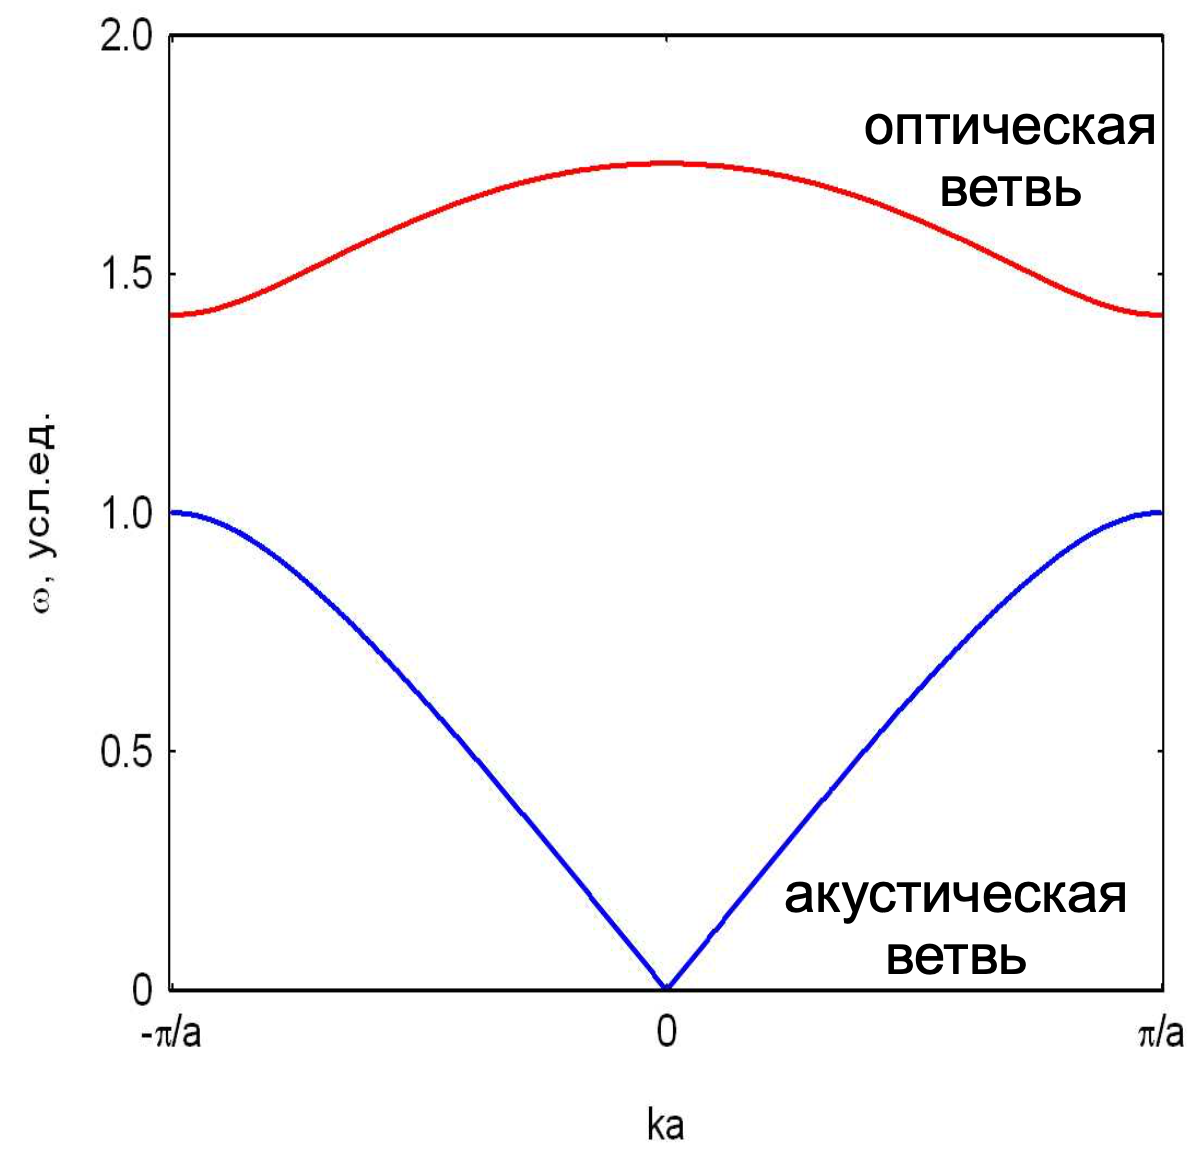
\includegraphics[width=0.8\textwidth]{2}
%	\caption{К вопросу №1}
%	\label{fig:1}
%\end{figure}
	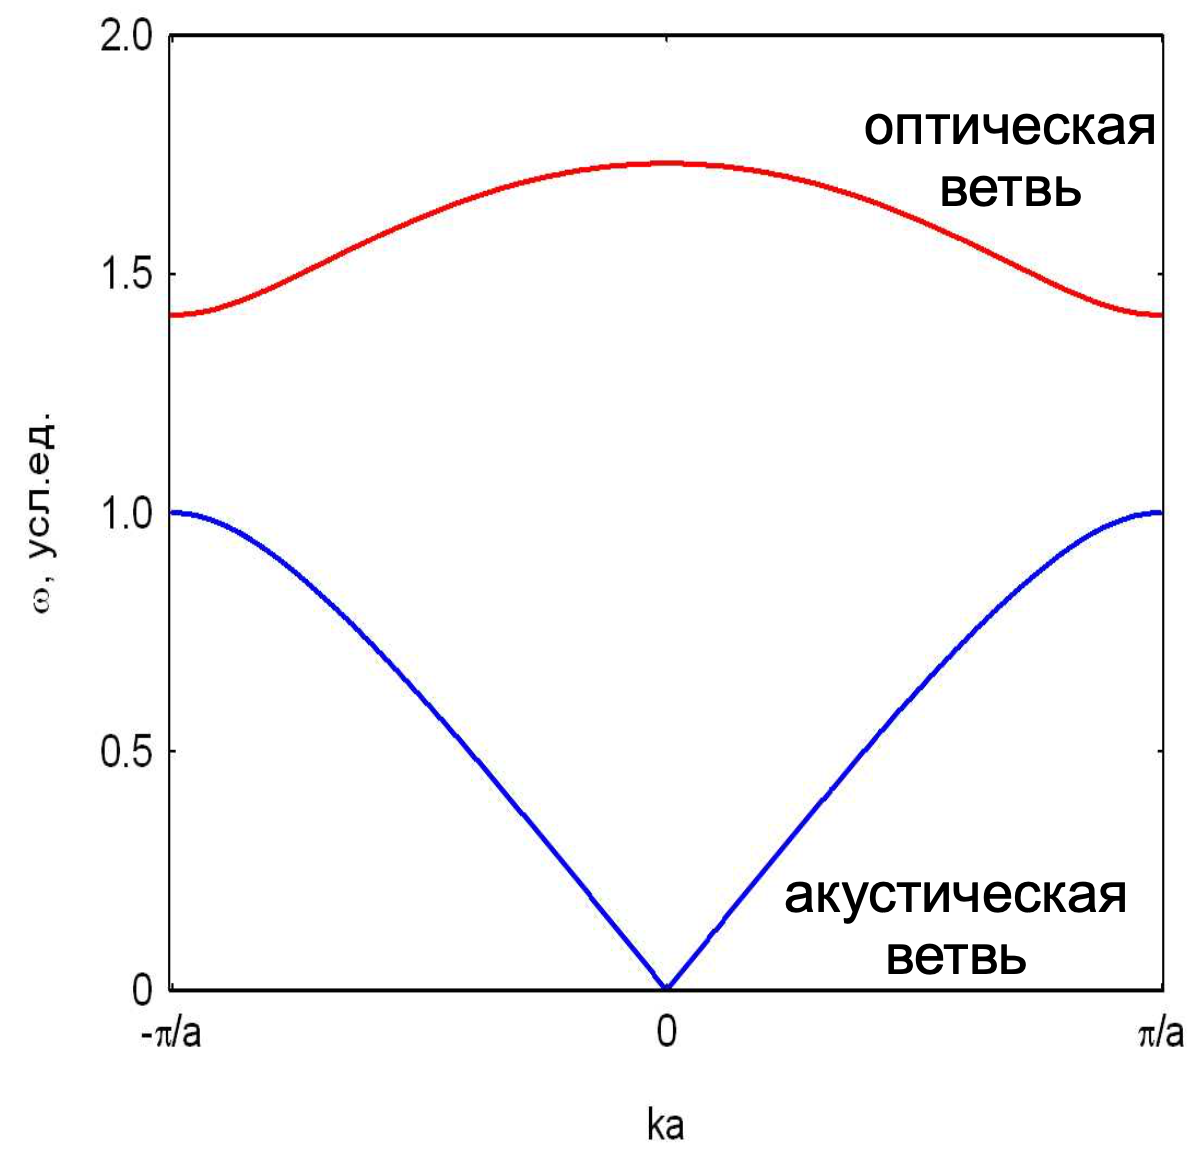
\includegraphics[width=\linewidth]{2}
\section{Определение векторов обратной решётки.}
Если $\mathbf{a},\ \mathbf{b},\ \mathbf{c}$ --- вектора трансляций обычной решётки, то вектора обратной решётки с точностью до циклической перестановки
\[
	\mathbf{a}^*=2\pi \frac{\mathbf{b}\times\mathbf{c}}{\mathbf{a}\cdot \left( \mathbf{b}\times \mathbf{c} \right) }
.\] 
\section{Определение первой зоны Бриллюэна, графическое построение первой зоны Бриллюэна для двумерной решётки.}
\begin{dfn*}
\emph{Первая зона Бриллюэна} --- это ячейка Вигнера-Зейца в пространстве обратной решётки.
\end{dfn*}
\begin{dfn*}
	\emph{Ячейка Вигнера-Зейтца} --- многогранник, высекаемый плоскостями, проходящими через середины отрезков, соединяющих узел решётки со всеми его соседями. 
\end{dfn*}
\emph{Графическое построение первой зоны Бриллюэна для двумерной прямоугольной решётки}
%\begin{figure}[ht]
%    \centering
%    \incfig{1}
%    \caption{К вопросу №2}
%    \label{fig:2}
%\end{figure}
\incfig{1}
\section{Связь границ зоны Бриллюэна с условием дифракции. Групповая скорость на границе зоны Бриллюэна.}
Волна, волновой вектор которой попадает на границу зоны Бриллюэна автоматически удовлетворяет условию дифракции, следовательно групповая скорость равна нулю.
\section{Закон Дебая (без коэффициента) и закон дю-Лонга и Пти для теплоёмкости твёрдого тела. Теплоёмкость металла (без коэффициента).}
Для низких температур теплоёмкость твёрдого тела описывается законом Дебая $C \propto T^3$, для высоких --- законом дю-Лонга и Пти $C=3R$. Теплоёмкость металла (вырожденного ферми-газа) имеет вид $C \propto \frac{T}{E_F}R$.
\section{Порядок величины дебаевской температуры, её связь со скоростью звука.}
Порядок величины 300 К. Имеет место следующая оценка:
\[
\Theta= \frac{\hbar  \omega_D}{k_B}=\frac{\hbar}{k_B}
k_D s\approx \frac{\hbar }{k_B} \frac{\pi}{a} s\propto s
.\] 
\section{Модель Друде-Лоренца: связь проводимости со временем пробега.}
\[
\sigma=\frac{ne^2 \tau}{m^*}
,\] 
где $\sigma$ --- проводимость,  $\tau$ --- время свободного пробега, $n$ --- концентрация электронов, $m^*$ --- эффективная масса электрона.
\section{Процессы, ограничивающие длину свободного пробега при низких температурах: рассеяние на дефектах и границах образца.}
\section{Распределение Ферми-Дирака, вырожденный электронный газ.}
Функция распределения для ферми-частиц:
\[
	n(E)=\frac{1}{e^{\frac{E-\mu}{T}}+1}
.\] 
Вырожденный ферми-газ (электроны в металле): $T\ll \mu$.
%\begin{figure}[htpb]
%	\centering
%	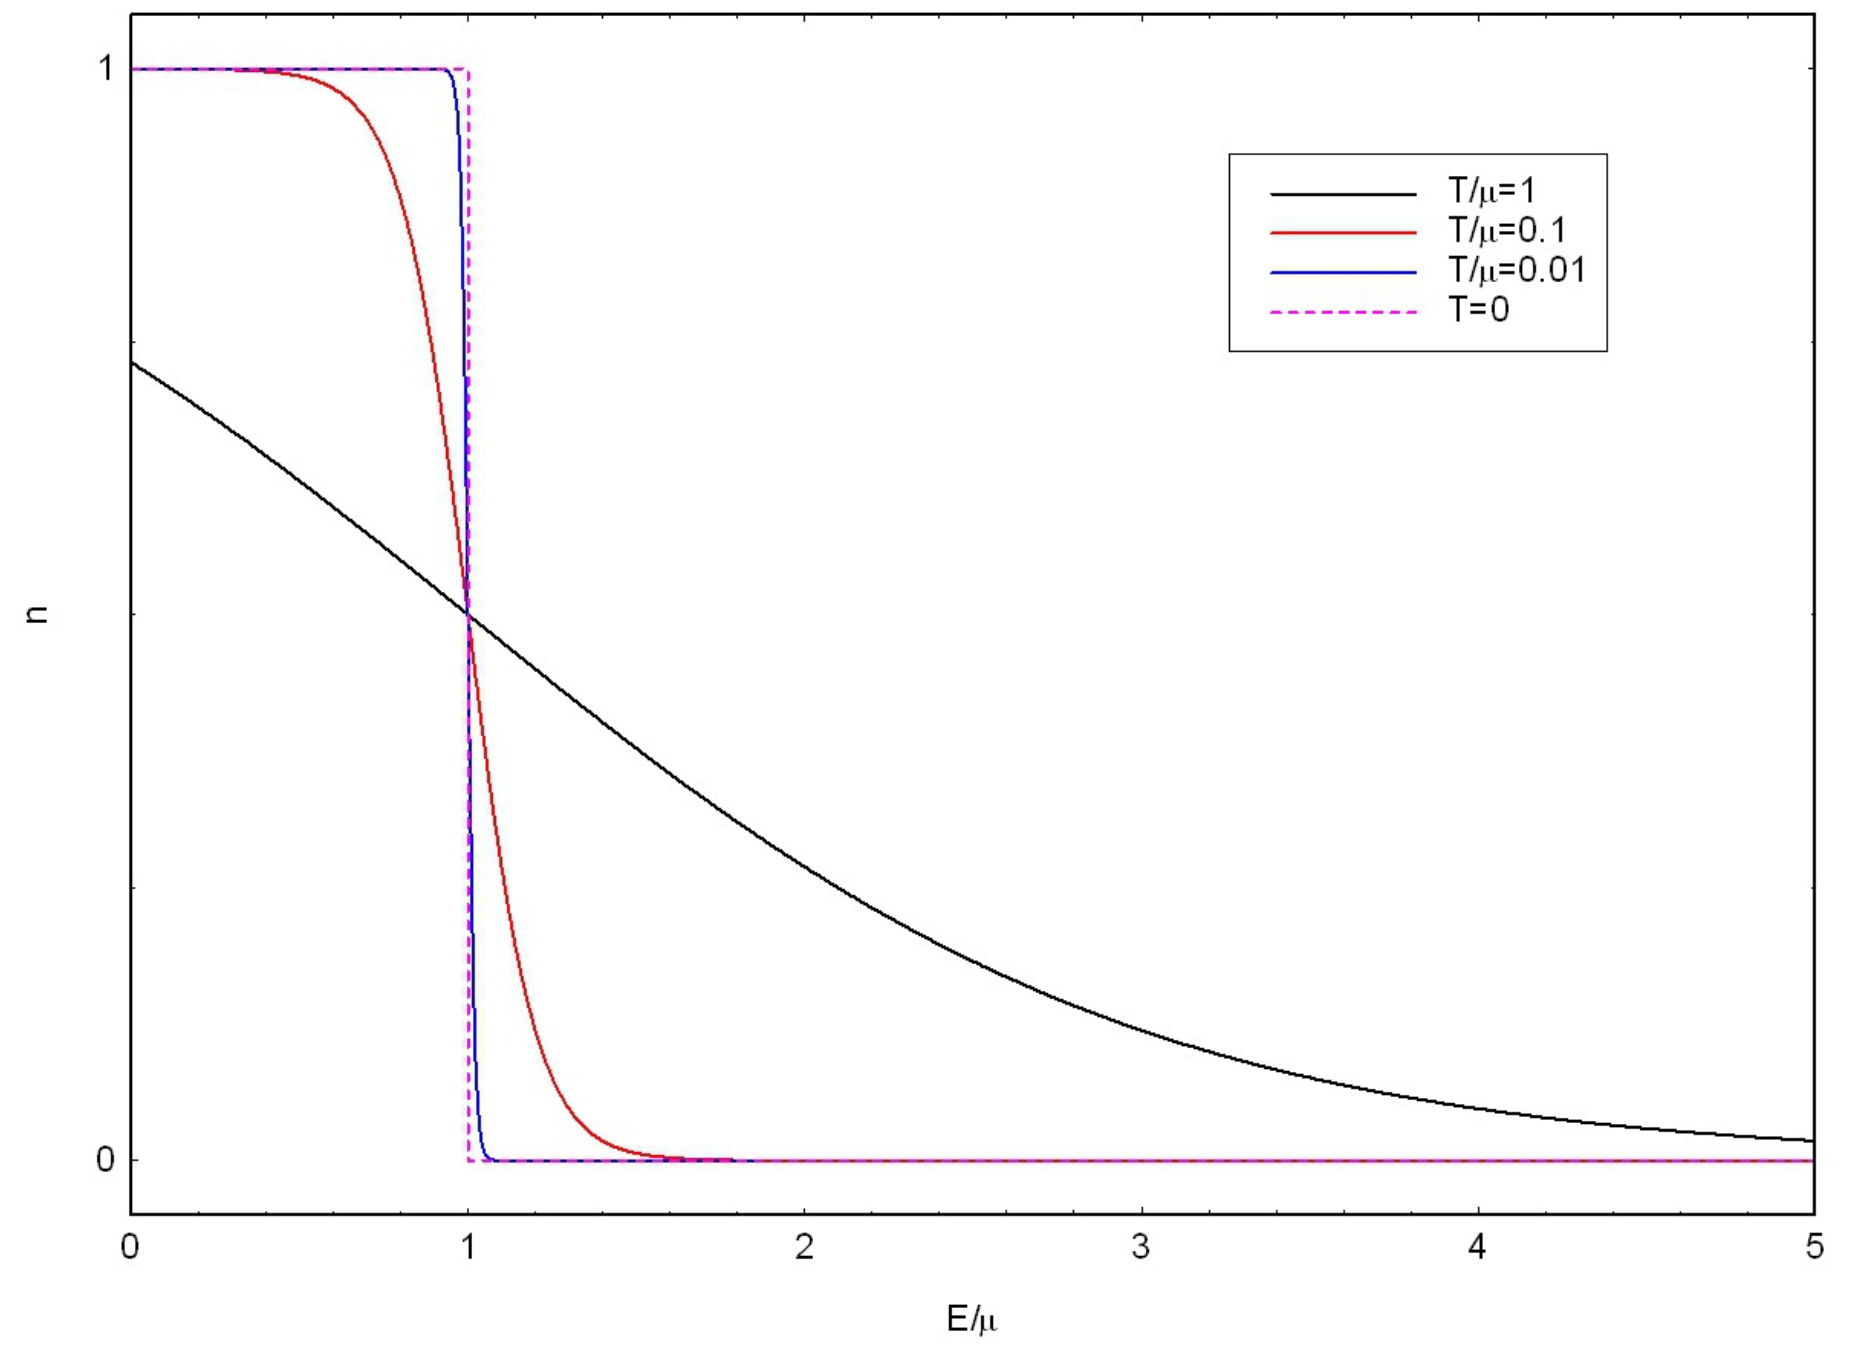
\includegraphics[width=0.8\textwidth]{3}
%	\caption{Функция распределения для ферми-частиц при разных значениях температуры.}
%	\label{fig:3}
%\end{figure}

\emph{Функция распределения для ферми-частиц при разных значениях температуры.}
	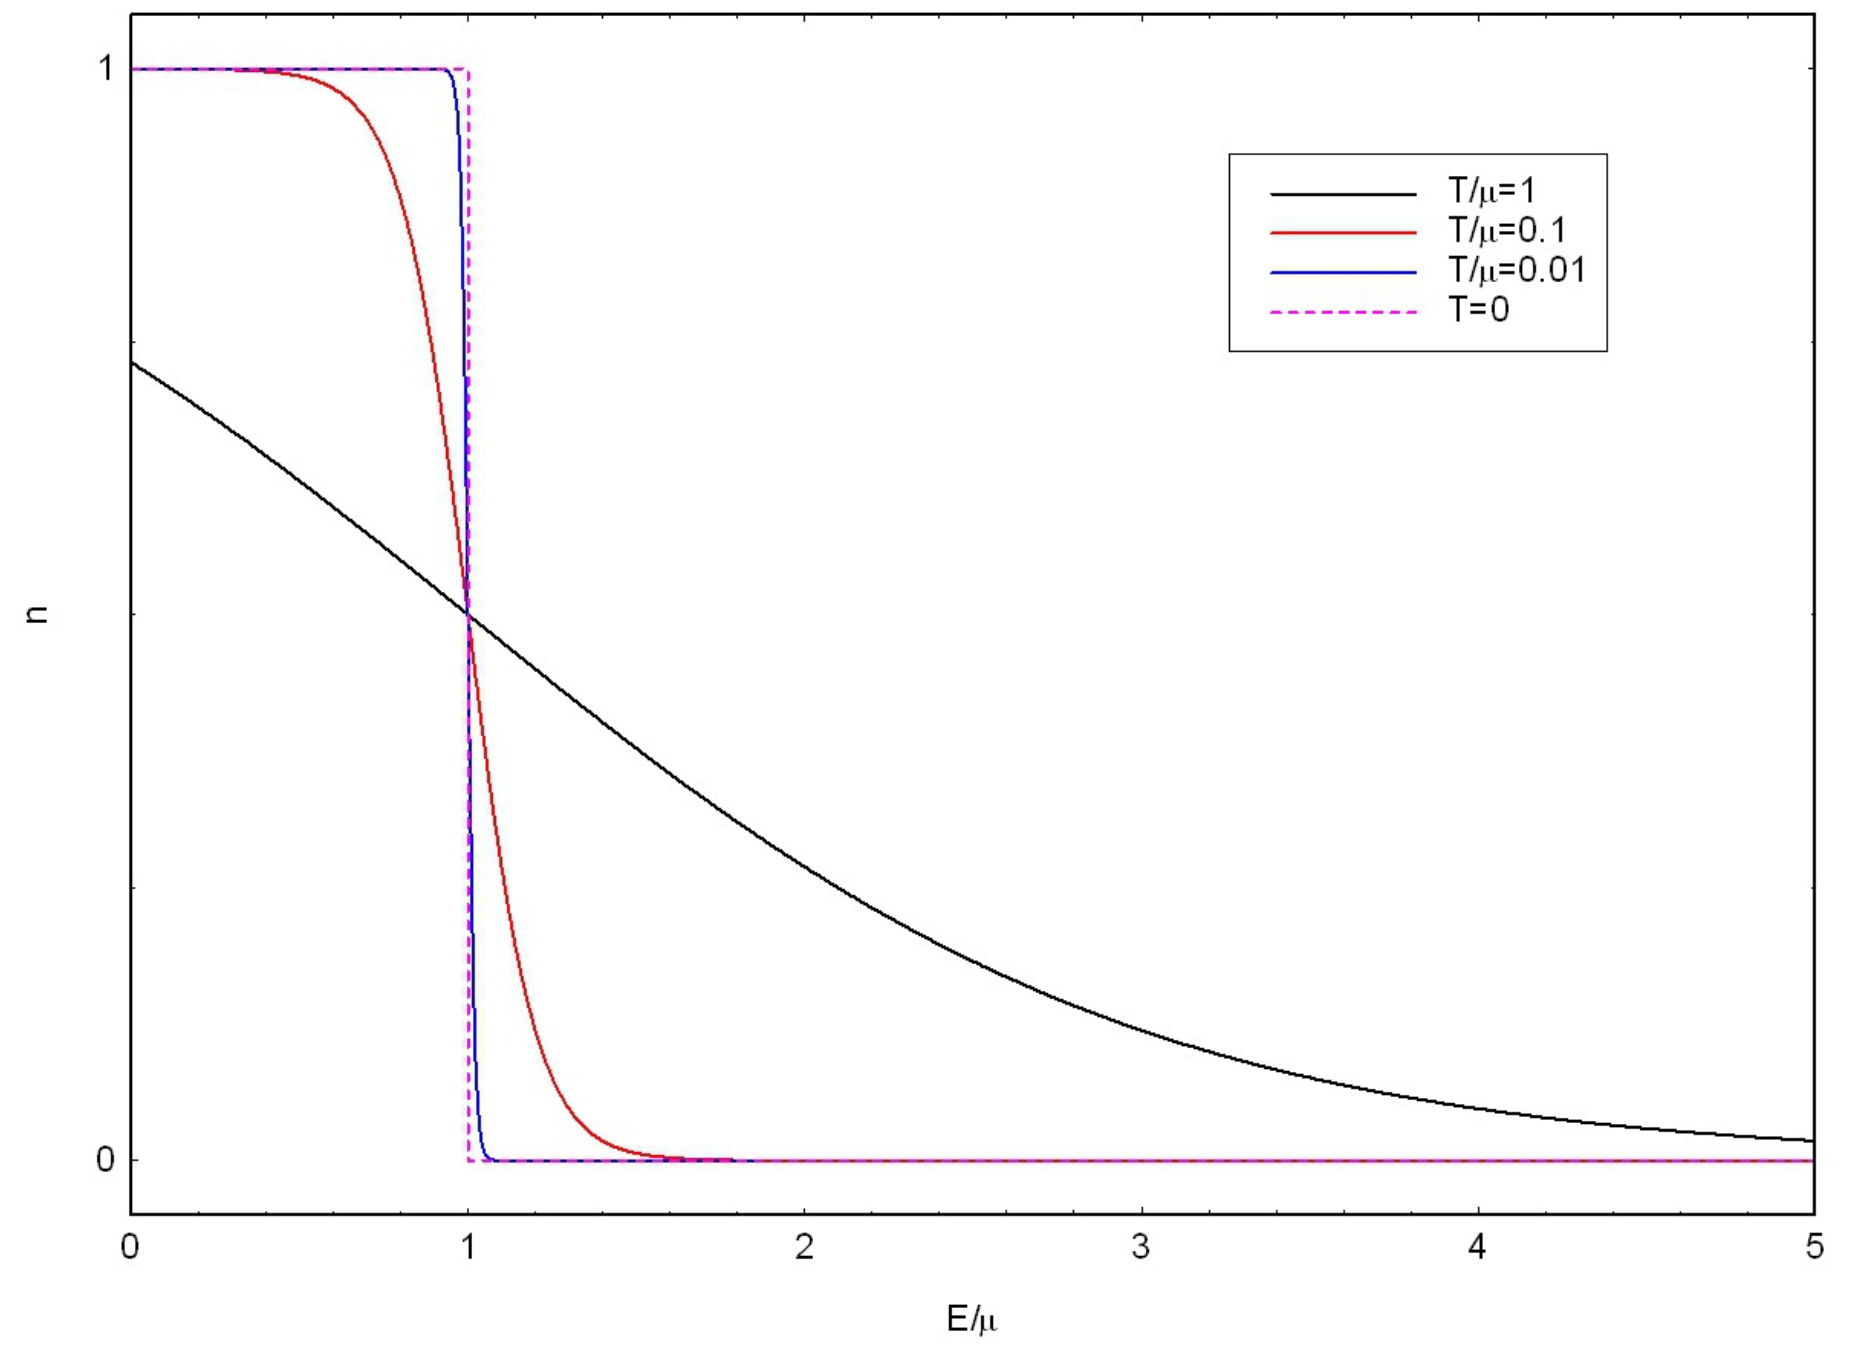
\includegraphics[width=\linewidth]{3}
\section{Вычисление энергии Ферми и импульса Ферми в трёхмерном случае, порядок величины для металлов.}
\[
	k_F=\sqrt[3]{3\pi^2 n}\approx \frac{3}{a}\approx 10^{10} \frac{1}{\text{м}},
\]
\[
E_F=\frac{\hbar ^2 k_F^2}{2m}
.\] 
\section{Связь проводимости с заполнением энергетических зон при $T=0$ (в одномерной модели).}
%\begin{figure}[htpb]
%	\centering
%	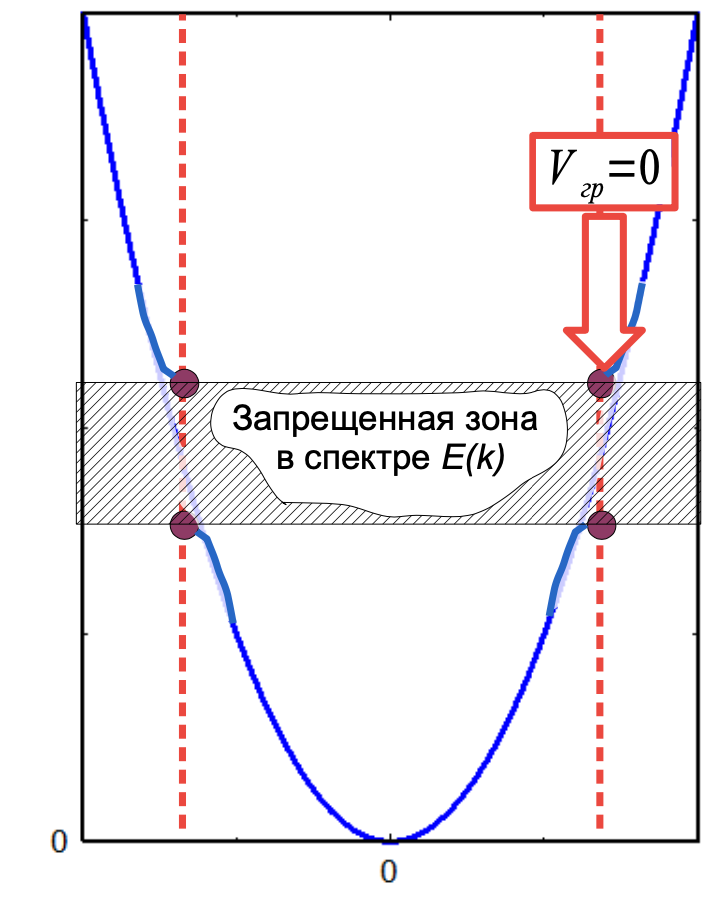
\includegraphics[width=0.8\textwidth]{4}
%	\caption{К вопросу №11}
%	\label{fig:4}
%\end{figure}
	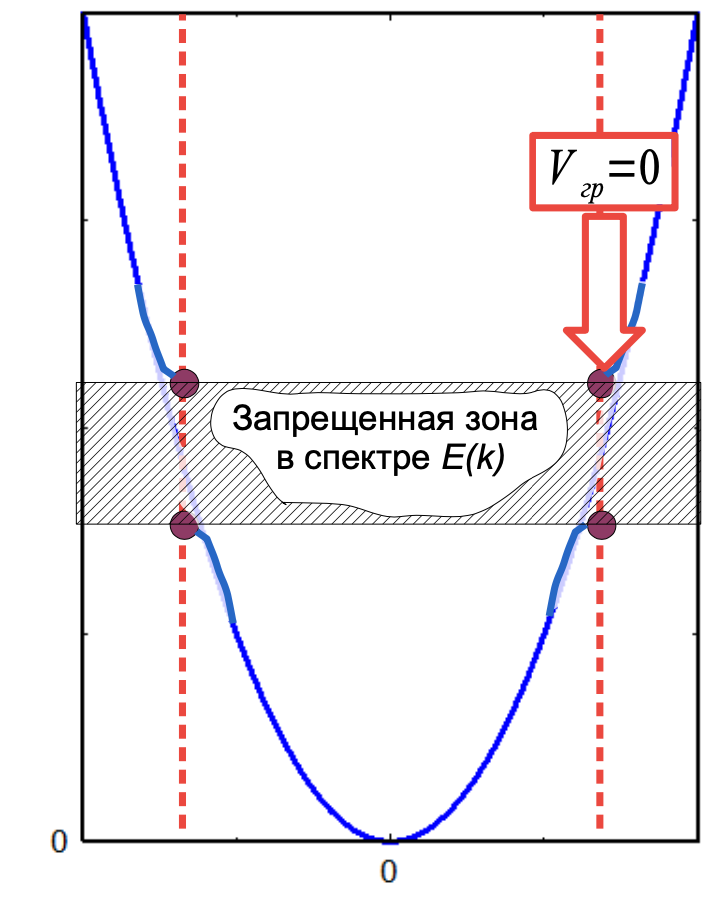
\includegraphics[width=\linewidth]{4}
\section{Положение химпотенциала в чистом и примесном (с единственным типом примеси) полупроводнике при $T=0$.}
%\begin{figure}[htpb]
%	\centering
%	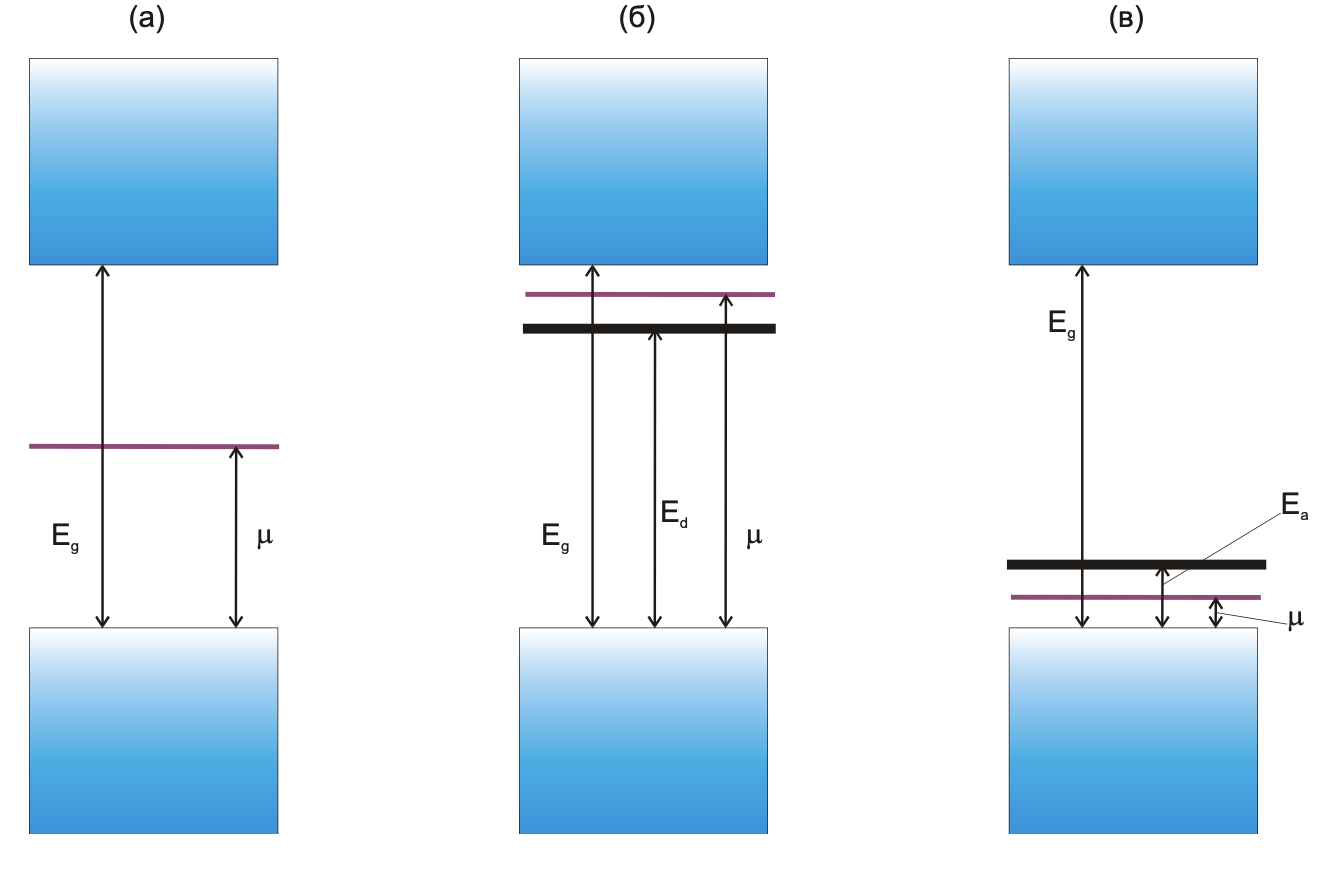
\includegraphics[width=0.8\textwidth]{5}
%	\caption{К вопросу №12. Упрощённое изображение зонной схемы полупроводника: (а) чистый полупроводник, (б) полупроводник с примесью донорного типа, (в) полупроводник с примесью акцепторного типа. — ширина запрещённой зоны, — уровень химпотенциала, — уровни донорной и акцепторной примеси. Положение химпотенциала показано для случая . Положение минимального уровня энергии электрона в вакууме не показано.}
%	\label{fig:5}
%\end{figure}
Упрощённое изображение зонной схемы полупроводника: (а) чистый полупроводник, (б) полупроводник с примесью донорного типа, (в) полупроводник с примесью акцепторного типа. — ширина запрещённой зоны, — уровень химпотенциала, — уровни донорной и акцепторной примеси. Положение химпотенциала показано для случая . Положение минимального уровня энергии электрона в вакууме не показано.
	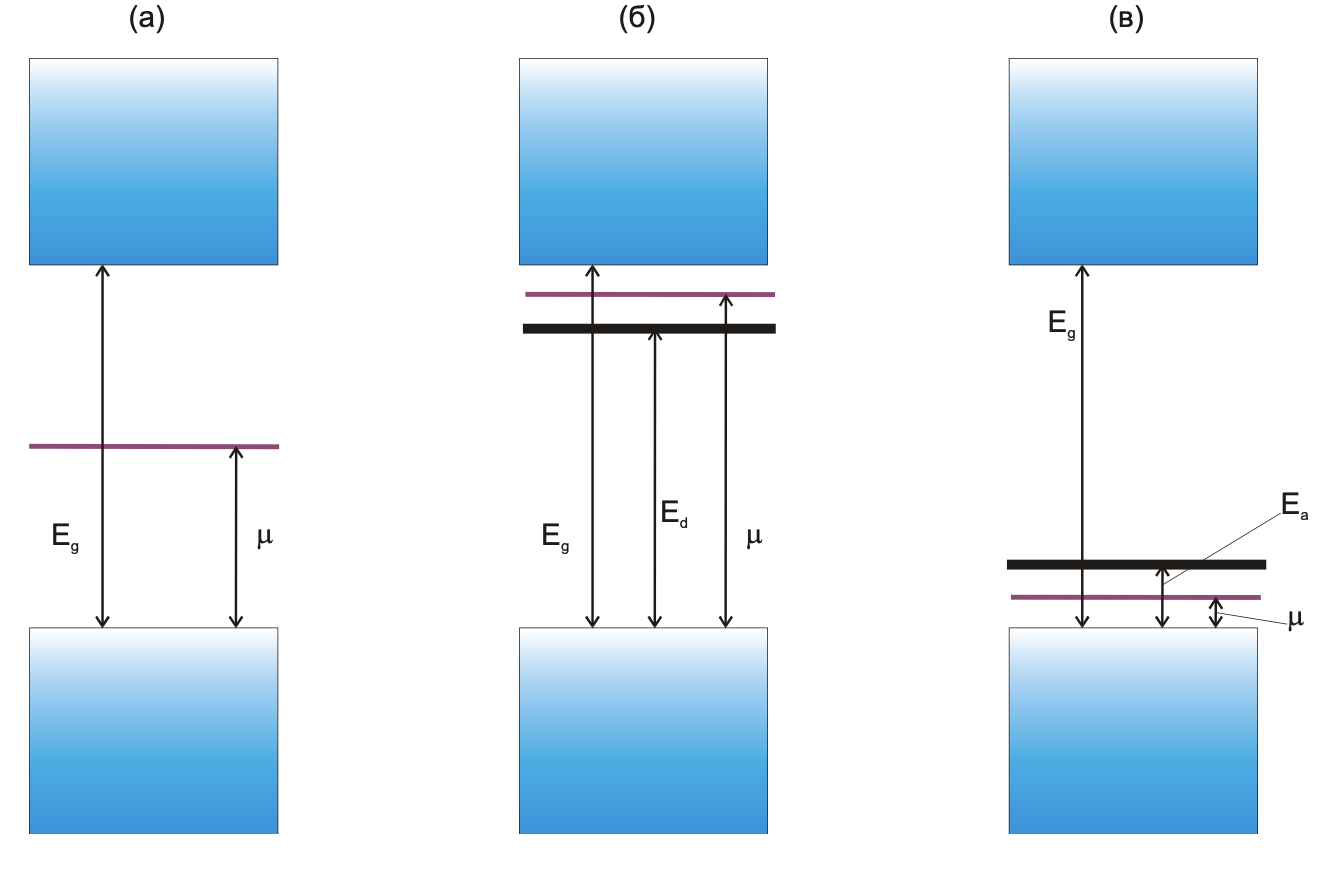
\includegraphics[width=\linewidth]{5}
\section{Основные экспериментальные факты о сверхпроводимости: эффект Мейсснера, критическое поле, щель в спектре.}
Полный эффект Мейснера: в малых полях сверхпроводник I рода полностью выталкивает из себя магнитное поле. Частичный эффект Мейснера: при поле выше некоторого порогового значения (но ниже поля полного разрушения сверхпроводимости) магнитное поле как-то проникает вглубь образца и намагниченность образца оказывается меньше намагниченности идеального диамагнетика.
%\begin{figure}[htpb]
%	\centering
%	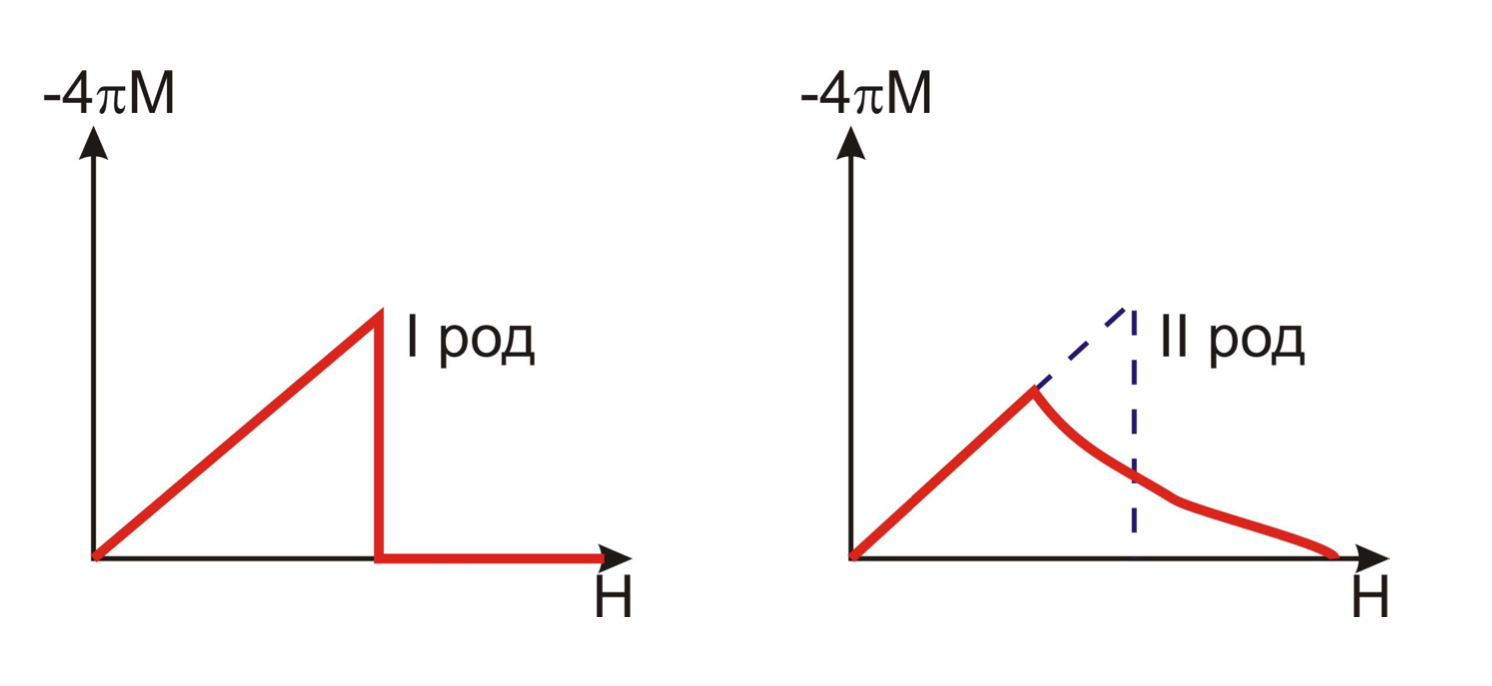
\includegraphics[width=0.8\textwidth]{6}
%	\caption{К вопросу №13. Эффект Мейсснера.}
%	\label{fig:6}
%\end{figure}

\emph{Эффект Мейсснера}:
	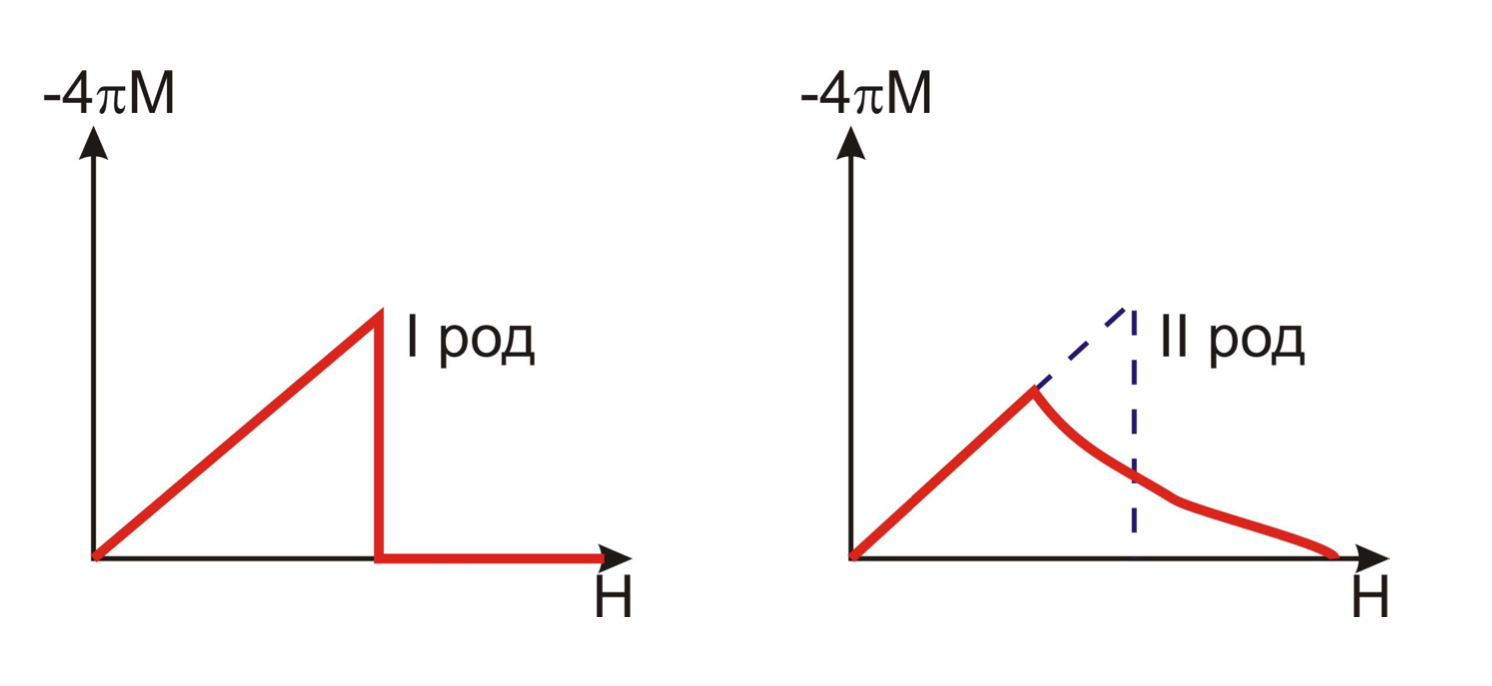
\includegraphics[width=\linewidth]{6}

%Щель в спектре сверхпроводника изображена на рис.~\ref{fig:7}.
%\begin{figure}[htpb]
%	\centering
%	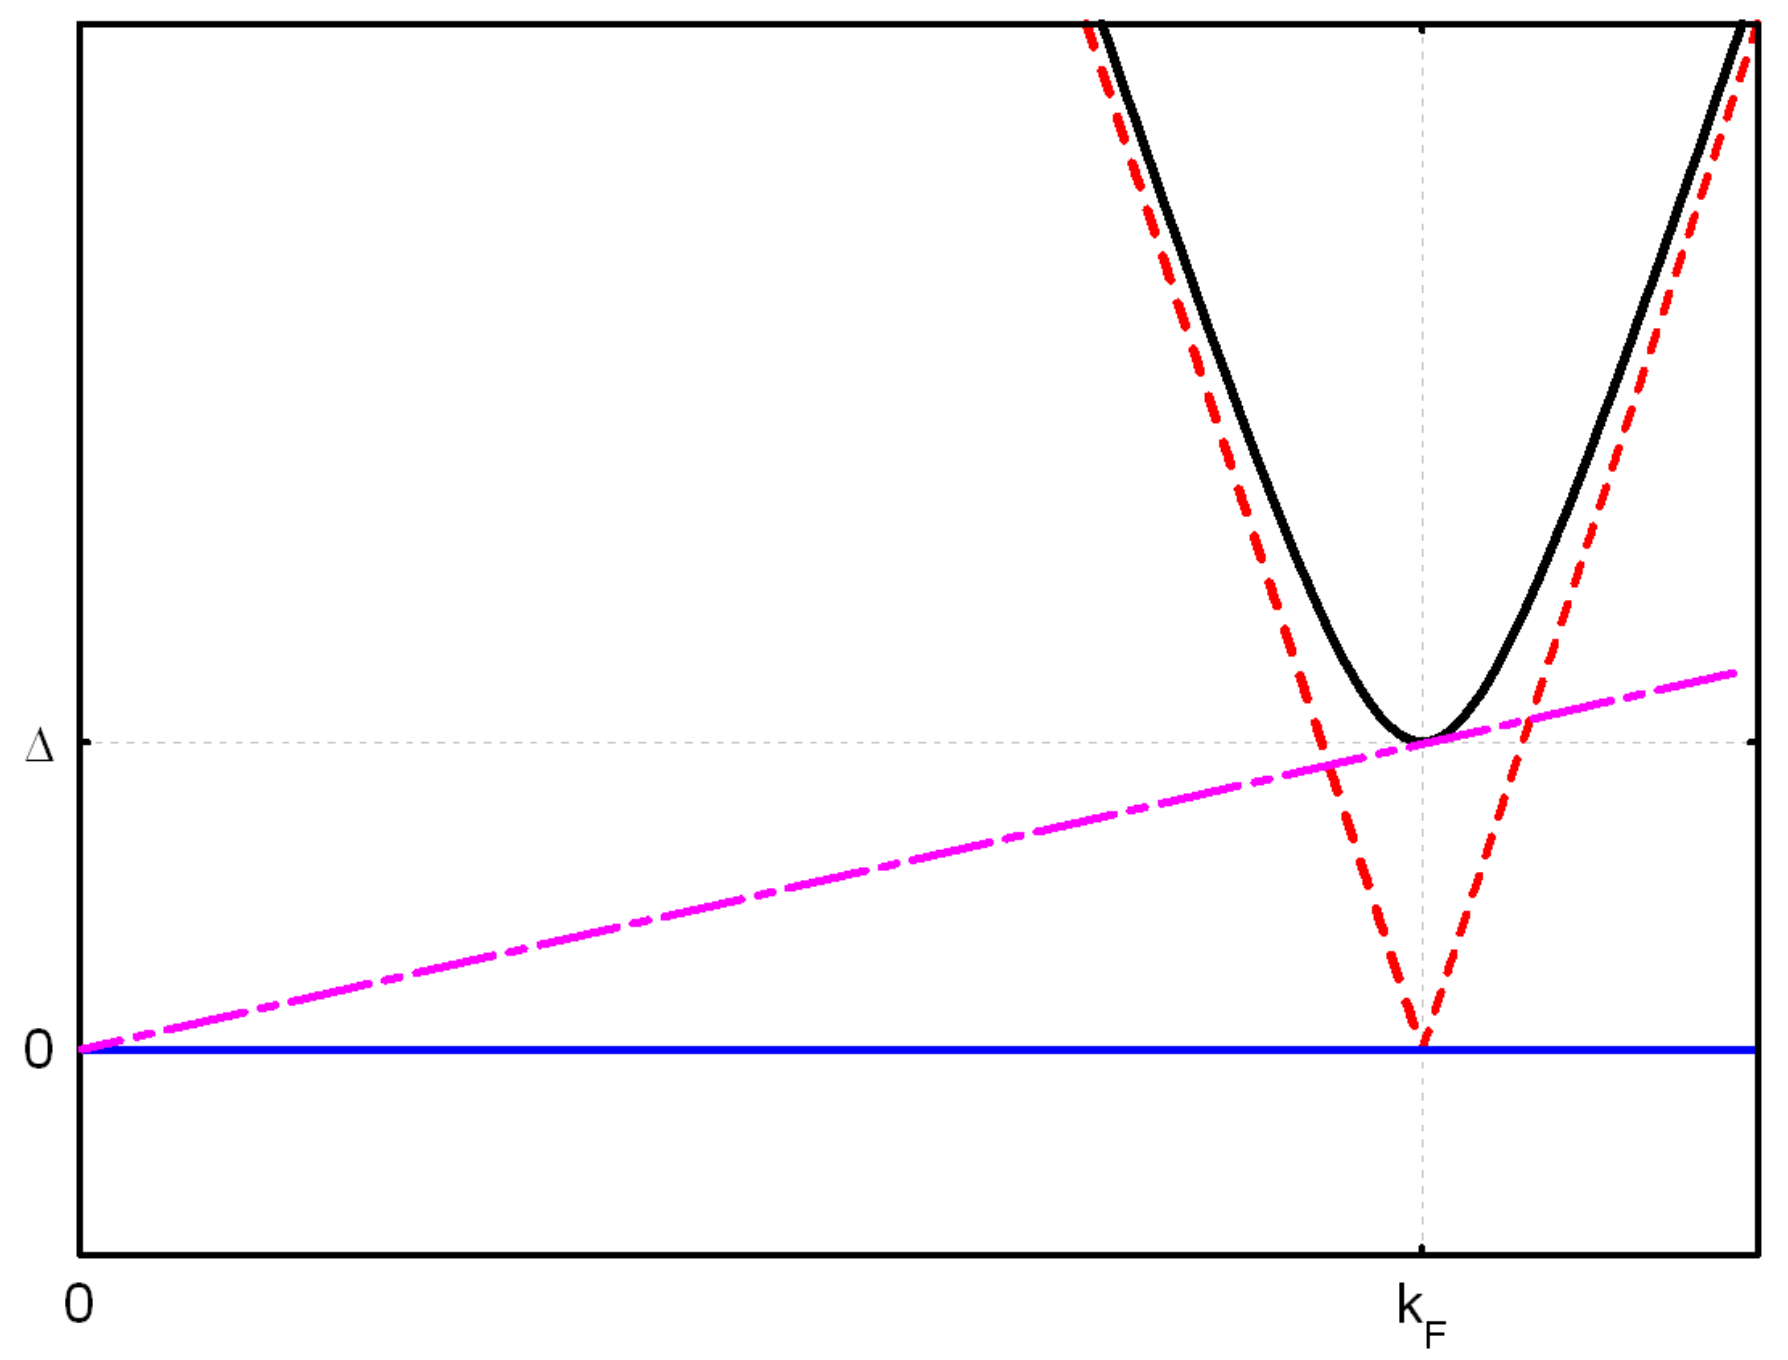
\includegraphics[width=0.8\textwidth]{7}
%	\caption{К вопросу №13. Спектр возбуждений в нормальном металле (пунктир) и сверхпроводнике (сплошная линия). $\Delta$ --- щель в спектре сверхпроводника.}
%	\label{fig:7}
%\end{figure}
	\emph{Спектр возбуждений в нормальном металле (пунктир) и сверхпроводнике (сплошная линия). $\Delta$ --- щель в спектре сверхпроводника.}
	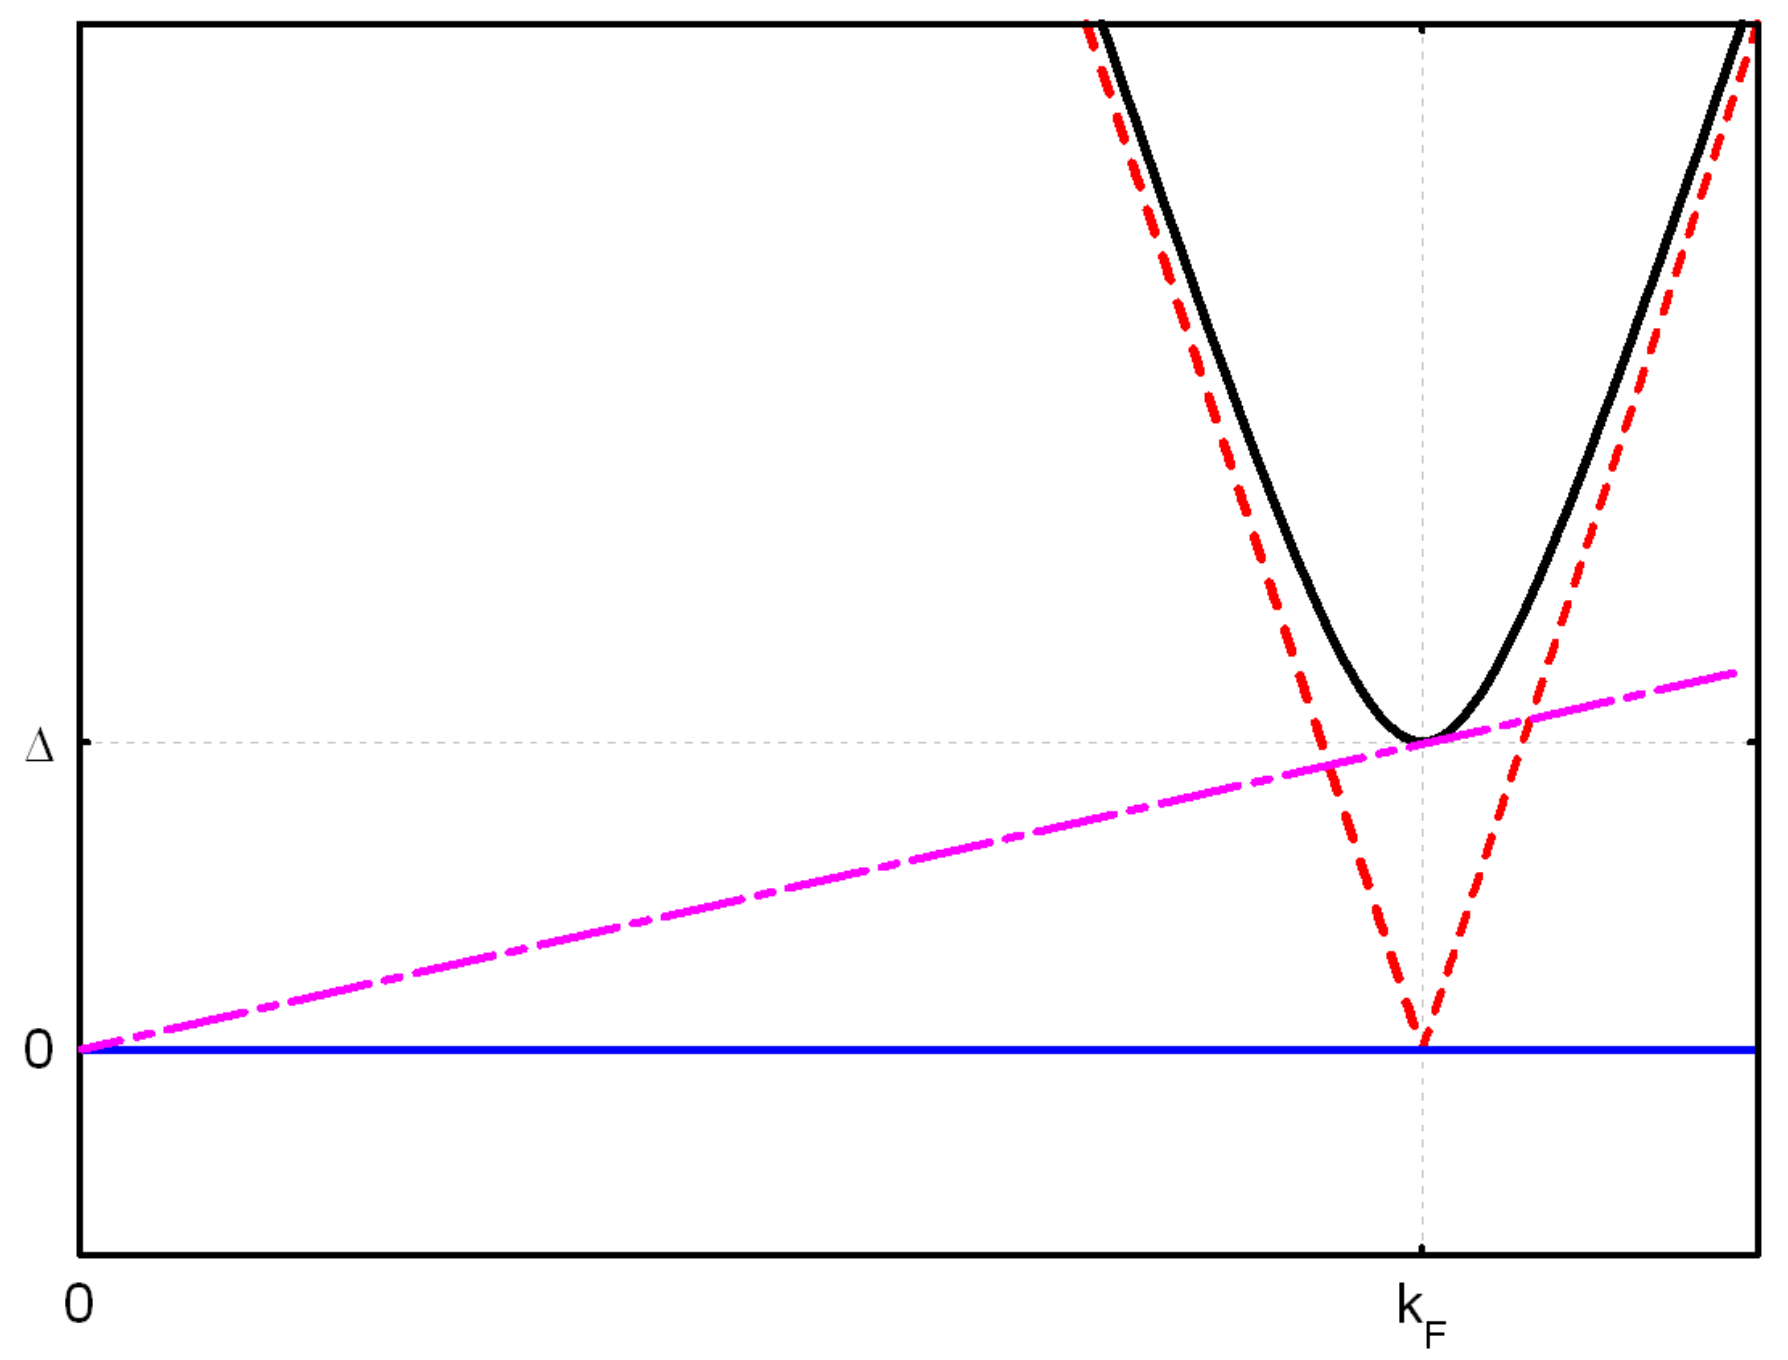
\includegraphics[width=\linewidth]{7}
\section{Роль обменного взаимодействия в формировании ферромагнетизма. Представление о фазовом переходе в ферромагнитное состояние.}
Гамильтониан обменного взаимодействия
\[
	\widehat{\operatorname{H}}_{ij}= \frac{1}{2}\sum_{i,j}^{} J_{ij}\widehat{\operatorname{\mathbf{S}}}_i \widehat{\operatorname{\mathbf{S}}}_j
,\] 
где сумма ведётся по соседям.
%\begin{figure}[htpb]
%	\centering
%	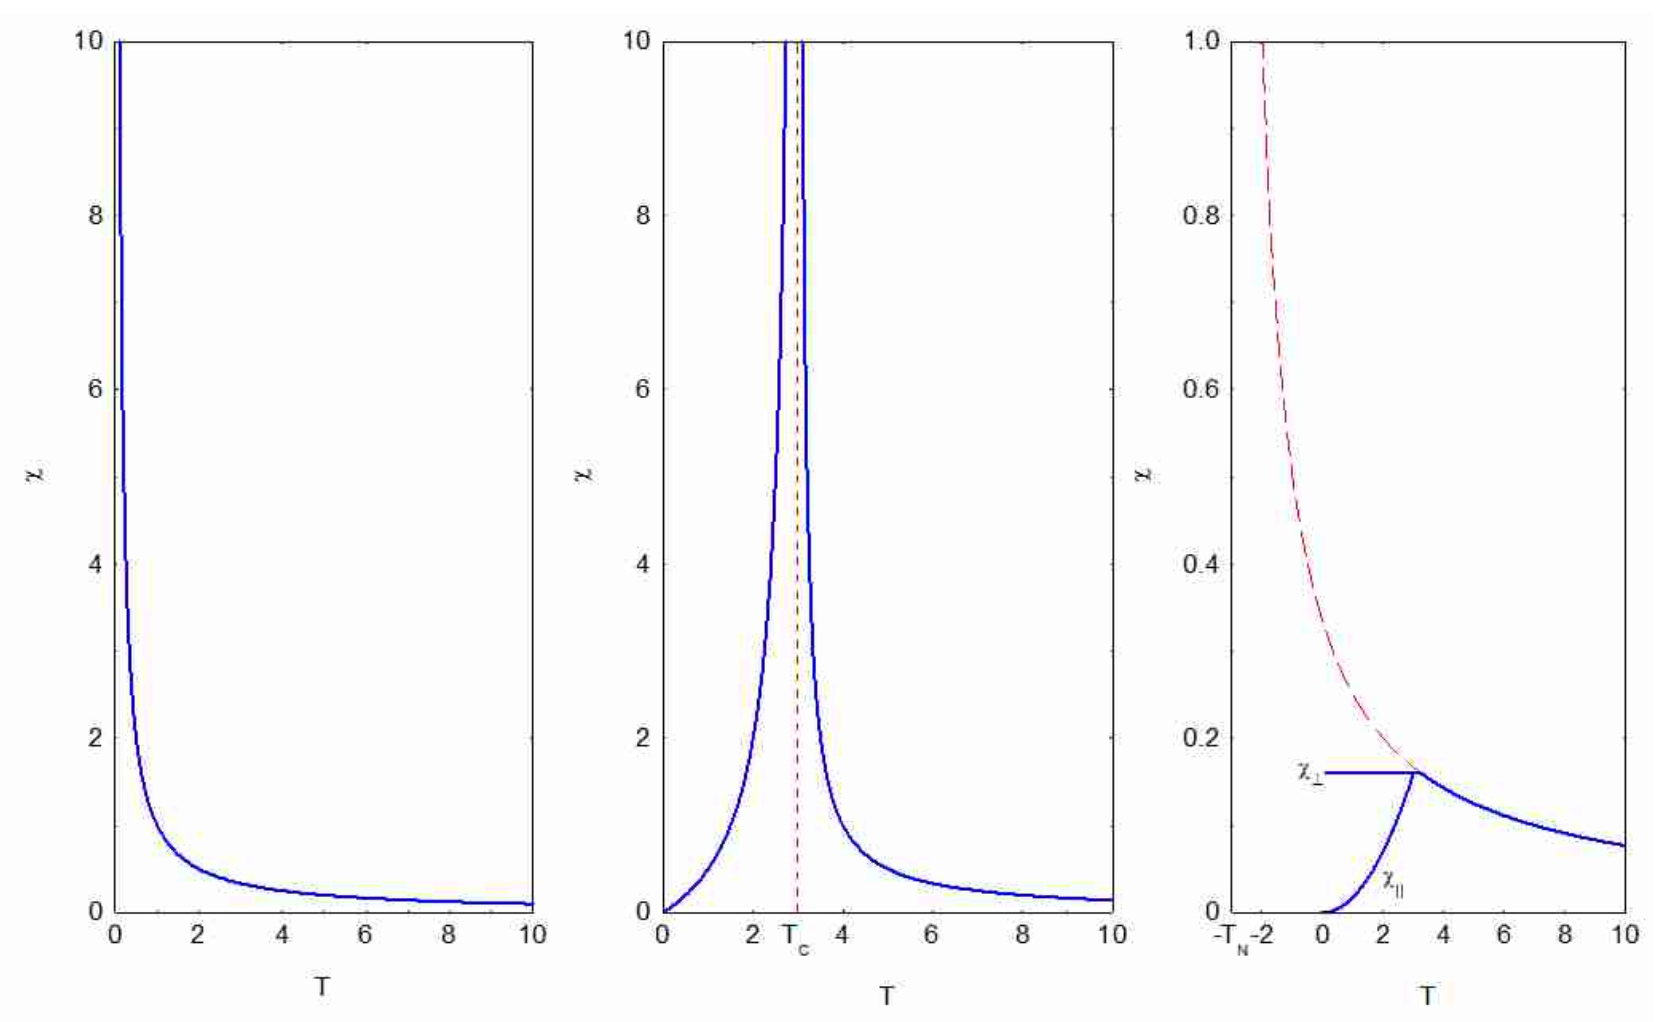
\includegraphics[width=0.8\textwidth]{8}
%	\caption{Схематическое изображение зависимости магнитной восприимчивости от температуры. Слева направо: парамагнетик (закон Кюри), ферромагнетик, антиферромагнетик. На графике для антиферромагнетика пунктиром построена кривая закона Кюри-Вейса.}
%	\label{fig:8}
%\end{figure}

\emph{Схематическое изображение зависимости магнитной восприимчивости от температуры. Слева направо: парамагнетик (закон Кюри), ферромагнетик, антиферромагнетик. На графике для антиферромагнетика пунктиром построена кривая закона Кюри-Вейса.}
	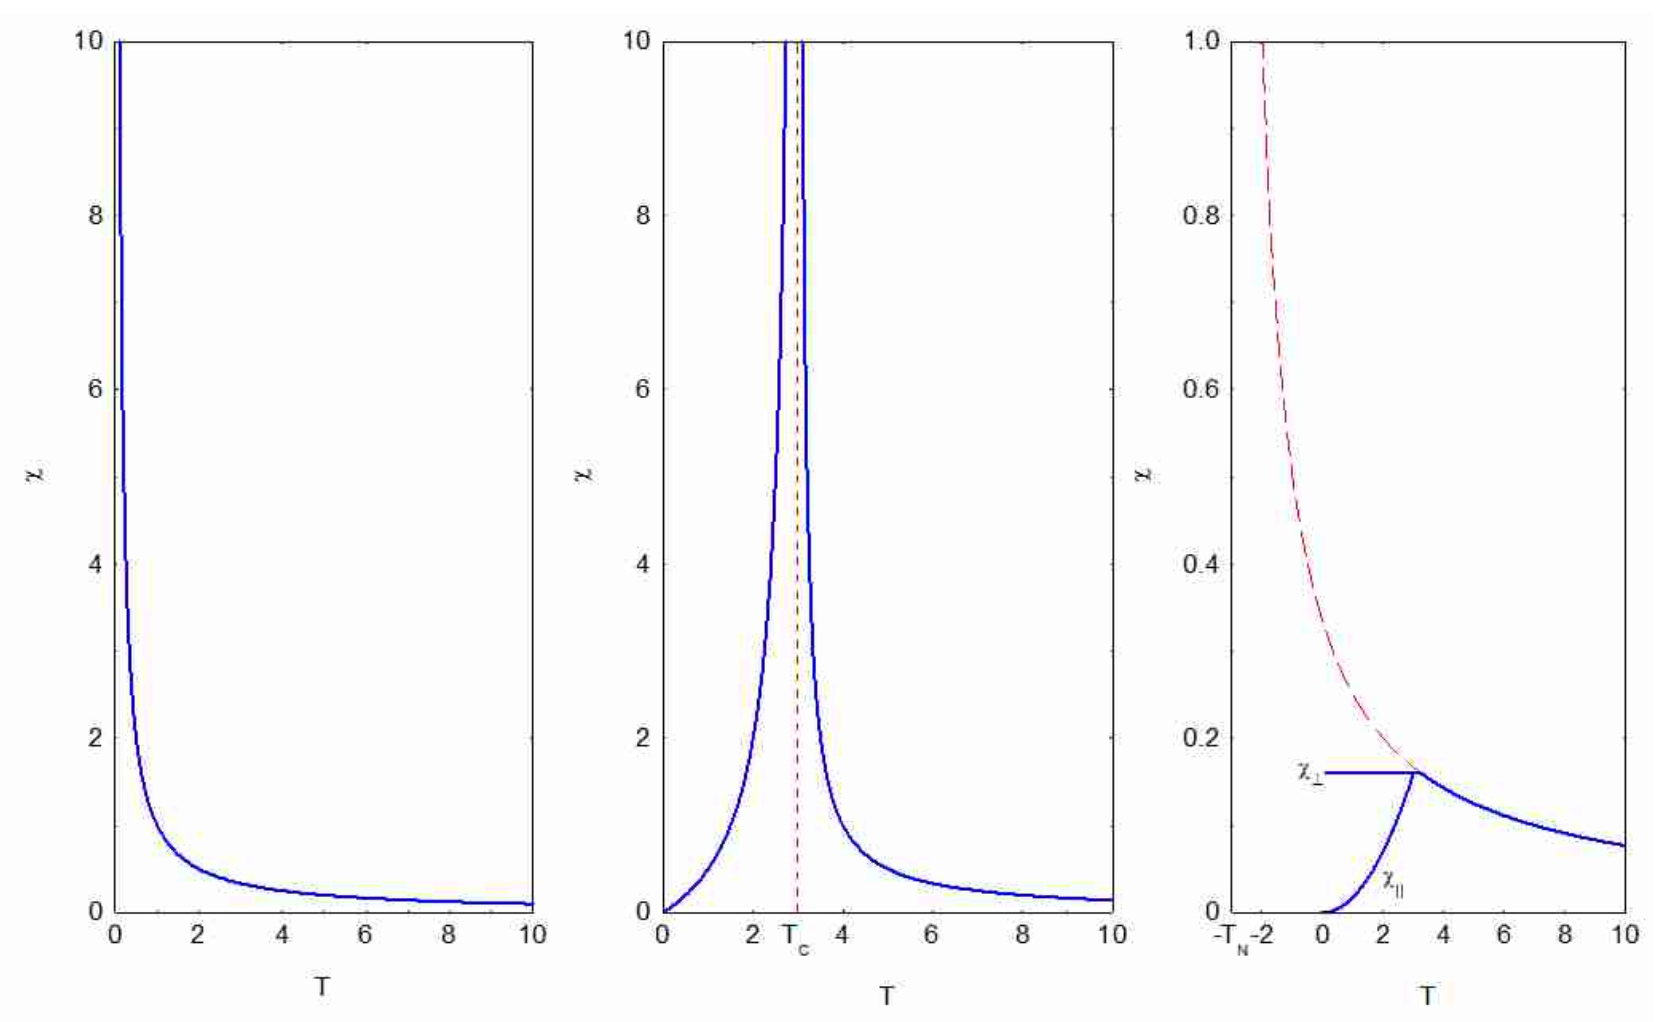
\includegraphics[width=\linewidth]{8}
%\begin{figure}[htpb]
%	\centering
%	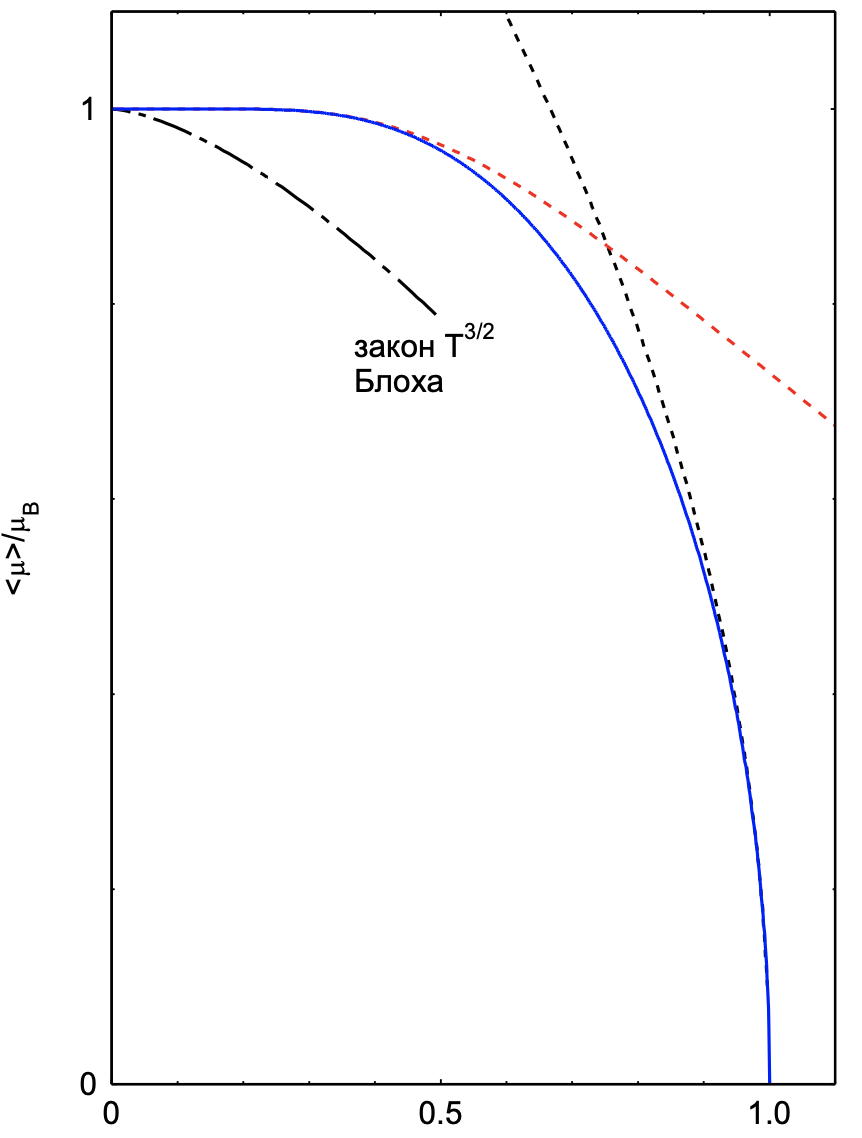
\includegraphics[width=0.8\textwidth]{9}
%	\caption{Сплошная линия - зависимость намагниченности подрешётки от температуры в модели молекулярного поля}
%	\label{fig:9}
%\end{figure}
\emph{Сплошная линия - зависимость намагниченности подрешётки от температуры в модели молекулярного поля}
	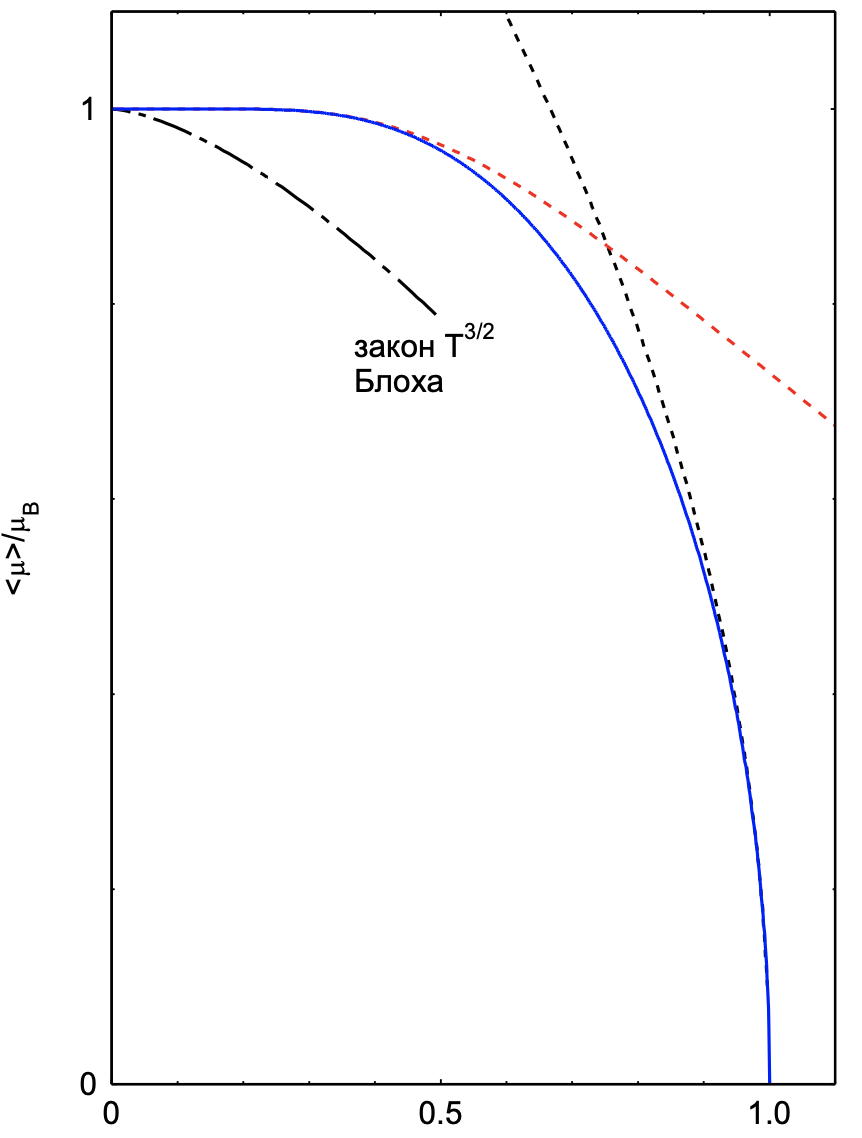
\includegraphics[width=\linewidth]{9}
\end{multicols}
\end{document}
